\subsection{M.PC.7 - Variazione del piano tra preventivo e consuntivo}
\begin{figure}[H]
    \centering
    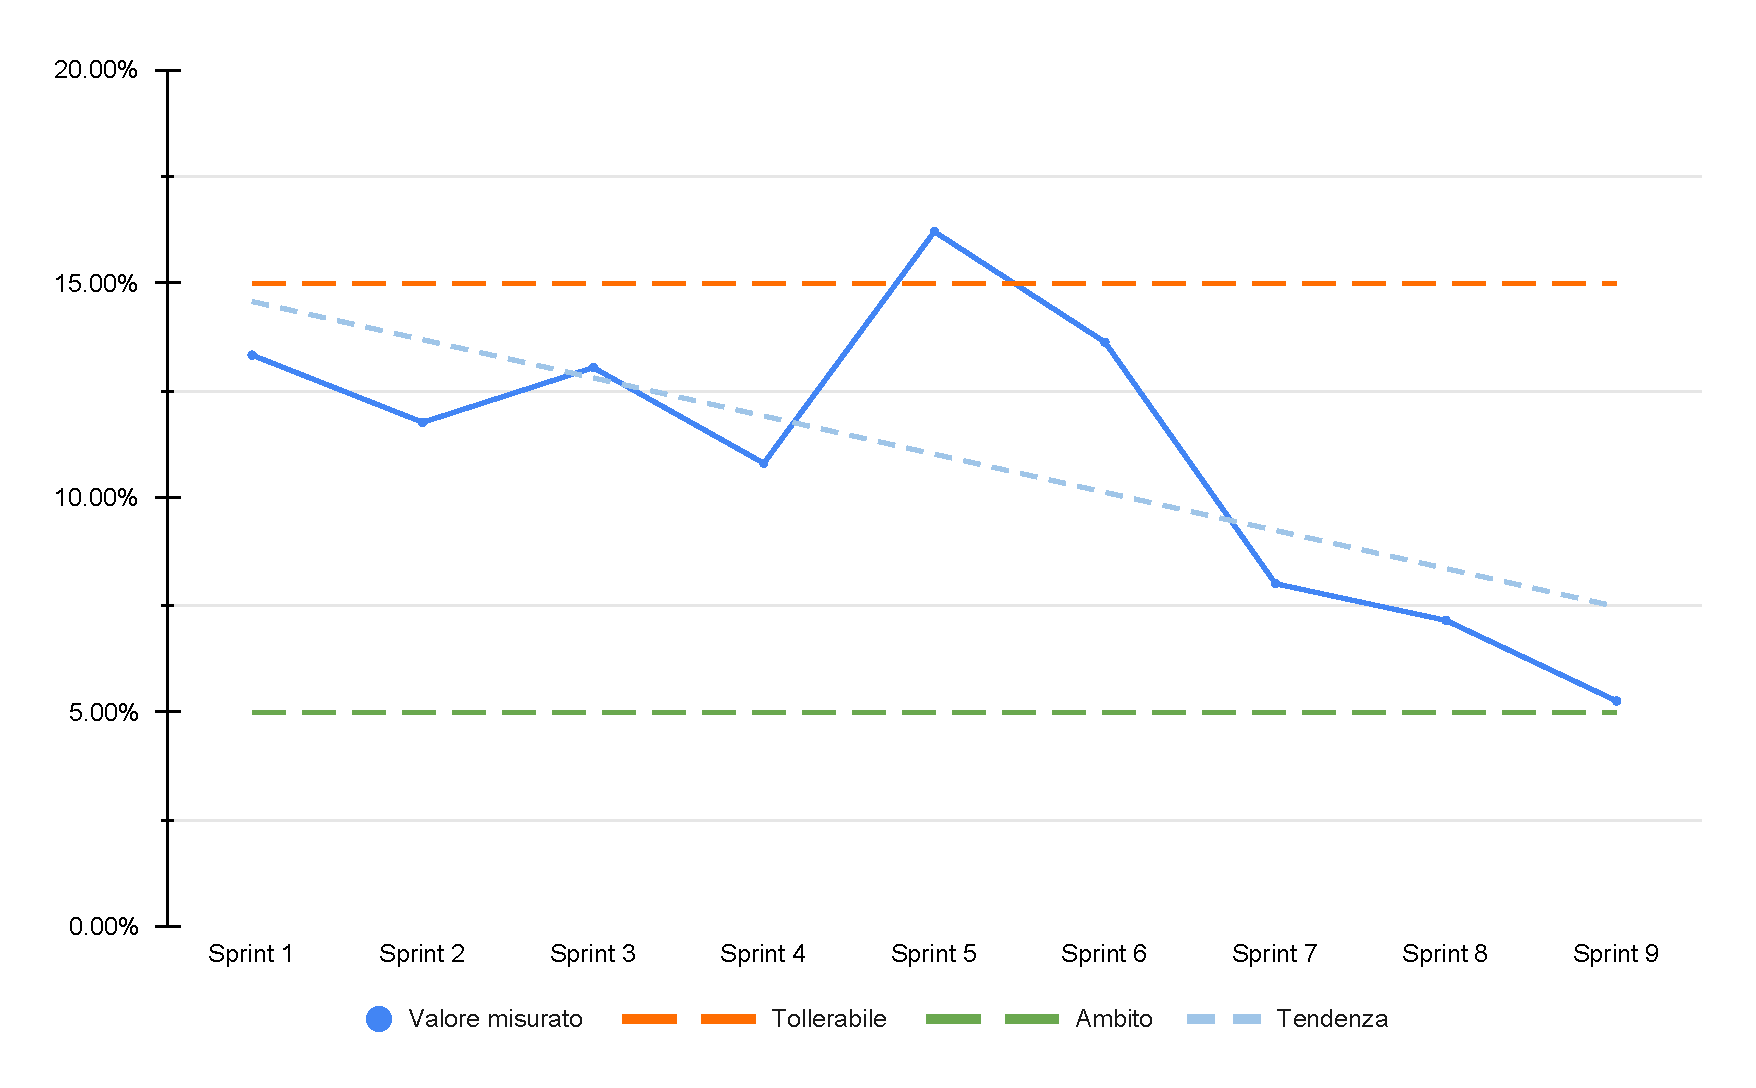
\includegraphics[width=\textwidth]{assets/variazione_task_completati.pdf}
    \caption{M.PC.7 - Variazione del piano tra preventivo e consuntivo}
\end{figure}

\par Il gruppo ha mantenuto un sano equilibrio nel rapporto tra le attività pianificate a inizio \glossario{sprint} e quelle completate. Il risultato è indice di una pianificazione iniziale discretamente accurata, anche se non ancora ottimale. Negli sprint iniziali (della durata di due settimane), il team ha faticato ad avvicinarsi al valore ambito; questo per via di un carico di lavoro eccessivo assegnato ad alcuni membri e ruoli di progetto. L’ampia durata degli sprint ha comportato una pianificazione non previdente e troppo ambiziosa. Nonostante ciò, la discrepanza tra i task pianificati e quelli completati è rimasta entro i parametri di accettabilità. Il picco in corrispondenza del quinto \glossario{sprint} è dovuto alla sua durata minore, per cui la pianificazione iniziale non è stata bilanciata adeguatamente. A partire dalla misura successiva si è tuttavia ricalibrato il carico di lavoro, rientrando nel range di tollerabilità. Superato il debito tecnico dovuto al cambio di tecnologie, il team è riuscito ad avvicinarsi al valore ambito.
